\documentclass[12pt,fleqn,answers]{exam}
\usepackage{pifont}
\usepackage{dingbat}
\usepackage{amsmath,amssymb}
\usepackage{epsfig}
\usepackage[colorlinks=true,linkcolor=black,anchorcolor=black,citecolor=black,filecolor=black,menucolor=black,runcolor=black,urlcolor=black]{hyperref}
\usepackage[letterpaper, margin=0.75in]{geometry}
\usepackage{tikz}
\usetikzlibrary{arrows}
\addpoints
\boxedpoints
\pointsinmargin
\pointname{pts}

\usepackage{pdfpages}
\usepackage[final]{microtype}
\usepackage[american]{babel}
\usepackage[T1]{fontenc}
\usepackage{fourier}
\usepackage{isomath}
\usepackage{upgreek,amsmath}
\usepackage{amssymb}

\newcommand{\dotprod}{\, {\scriptzcriptztyle
    \stackrel{\bullet}{{}}}\,}

\newcommand{\reals}{\mathbf{R}}
\newcommand{\lub}{\mathrm{lub}} 
\newcommand{\glb}{\mathrm{glb}} 
\newcommand{\complex}{\mathbf{C}}
\newcommand{\dom}{\mbox{dom}}
\newcommand{\range}{\mbox{range}}
\newcommand{\cover}{{\mathcal C}}
\newcommand{\integers}{\mathbf{Z}}
\newcommand{\vi}{\, \mathbf{i}}
\newcommand{\vj}{\, \mathbf{j}}
\newcommand{\vk}{\, \mathbf{k}}
\newcommand{\bi}{\, \mathbf{i}}
\newcommand{\bj}{\, \mathbf{j}}
\newcommand{\bk}{\, \mathbf{k}}
\newcommand{\dist}{\, \mathrm{dist}}
\DeclareMathOperator{\Arg}{\mathrm{Arg}}
\DeclareMathOperator{\Ln}{\mathrm{Ln}}
\newcommand{\imag}{\, \mathrm{i}}

\usepackage{xcolor}
\shadedsolutions
\definecolor{SolutionColor}{rgb}{0.95,0.95,0.95}

\usepackage{graphicx}
\newcommand\AM{{\sc am}}
\newcommand\PM{{\sc pm}}
     
%\usepackage{twemojis}
\newcommand{\quiz}{7}
\newcommand{\term}{Spring}
\newcommand{\due}{9:55 \AM}
\newcommand{\class}{MATH 102}

\usepackage{siunitx}
\begin{document}
\large
\vspace{0.1in}
\noindent\makebox[3.0truein][l]{\textbf{\class, \term \/ \the\year}}
\textbf{Name:} \hrulefill \\
\noindent \makebox[3.0truein][l]{\textbf{In class work \quiz}}
\textbf{Row and Seat}:\hrulefill\\
\vspace{0.1in}

\begin{quote}
``\emph{Some things will drop out of the 
public eye and go away, but there will always be science, engineering, 
and technology. And there will always, always be mathematics.}'' \hfill {\sc Katherine Johnston}
\end{quote}
\noindent  In class work  \quiz\/  has questions 1 through  \numquestions \/ with a total of  \numpoints\/  points.   
 This assignment is due at the end of the class period (\due).
This assignment is printed on \textbf{both} sides of the paper.
\vspace{0.1in}

$\num[input-exponent-markers ={d,b}]{-3.4b-20}$

\begin{questions} 

   
  \question Follow these steps to solve the inequality $x^2 - x \geq 12$.

  \begin{parts}

    \part [2] \emph{Solve} the equation $x^2 -x = 12$.

    \begin{solution}[2.0in]
      \begin{align*}
        \left[x^2 -x = 12 \right] &= \left[x^2 -x -12 =0 \right]  &\mbox{(subtract 12)}\\
                    &= \left[(x-4)(x+3) =0 \right]  &\mbox{(factor)}\\
                    &= \left[x=4 \mbox{ or } x=-3  \right] & \mbox{(teacher's pet fact)}      
      \end{align*}

    \end{solution}

    \part [2] Check that \emph{both of your solutions are correct} by 
    pasting them into the equation $x^2 -x = 12$.

    \begin{solution}[2.0in]
      Pasting in $x \to 4$ into $x^2 -x = 12$ gives
      \begin{equation*}
          \left[4^2 - 4 = 12\right] = [12=12] = \mbox{True!}
      \end{equation*}
      And Pasting in $x \to -3$ into $x^2 -x = 12$ gives
      \begin{equation*}
          \left[(-3)^2 + 3 = 12\right] = [12=12] = \mbox{True!}
      \end{equation*}

    \end{solution}

    \part [2] Put both of your solutions on a \emph{number line}, correctly
    ordered from \emph{least to greatest}.

    \begin{solution}%[1.0in]

      \usetikzlibrary{arrows}
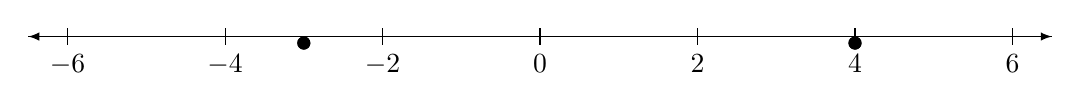
\begin{tikzpicture}
\draw[latex-] (-6.5,0) -- (6.5,0) ;
\draw[-latex] (-6.5,0) -- (6.5,0) ;
\foreach \x in  {-6,-4,-2,0,2,4,6}
\draw[shift={(\x,0)},color=black] (0pt,3pt) -- (0pt,-3pt);
\foreach \x in {-6,-4,-2,0,2,4,6}
\draw[shift={(\x,0)},color=black] (0pt,0pt) -- (0pt,-3pt) node[below] 
{$\x$};
%\draw[*-o] (-3,-3) -- (-3,-3)
\draw[*-o] (-3,0);
\draw[*-o] (4,0);
\end{tikzpicture}

    \end{solution}

    \vfill
    \newpage

    \part [2] Make a \emph{table} of the intervals determined by the number line 
    from the previous part, the test points, and the
    value of $x^2 - x \geq 12$ at each test point.
        
    \begin{solution}[4.0in]

      \begin{tabular}{|c|c|c|c|} \hline \hline 
        \textbf{Interval} &  $\mathbf{x}$  & $\mathbf{x^2 -x \geq 12}$  & \textbf{true or false}\\ \hline 
        $((-\infty,-3)$  & -4 &  $(-4)^2 + 4 \geq 12 $ & true \\  \hline 
        $((-3,4)$  & 0 &  $0^2 + 0 \geq  12 $  &false \\ \hline 
        $((4, \infty)$  & 5 &  $5^2 + 4 \geq 12 $ & true  \\ \hline        
      \end{tabular}

    \end{solution}


    \part [2] Finish the sentence:  The solution set is
    $(-\infty, -3] \cup [4 ,\infty)$. 
    
    We include the endpoints in each interval (use a bracket, not a paren) because we're
    solving $x^2 - x \geq 12$. And that allows equality. Here in 
    a bit, this rule will be modified.

   
  \end{parts}
\end{questions}
\end{document}
